\documentclass{exam}
\usepackage[utf8]{inputenc}
\usepackage{lmodern}
\usepackage{microtype}

% \usepackage[parfill]{parskip}
\usepackage[dvipsnames]{xcolor}
\usepackage{amsmath}
\usepackage{amsfonts}
\usepackage{amsthm}
\usepackage{siunitx}
\DeclareSIUnit\year{yr}
\DeclareSIUnit\foot{ft}
\DeclareSIUnit\litre{\liter}

\usepackage{skull}

\usepackage{pgfplots}
\usepgfplotslibrary{polar}
\pgfplotsset{compat=1.11}
\usepgfplotslibrary{statistics}
\usepackage{graphicx}
\usepackage{sidecap}
\sidecaptionvpos{figure}{c}
\usepackage{float}
\usepackage{gensymb}
\usepackage{tkz-euclide}
\usetkzobj{all}
\usepackage{commath}
\usepackage{hyperref}
\usepackage{enumitem}
\usepackage{wasysym}
\usepackage{multicol}
\usepackage{mathtools}
\usepackage{tcolorbox}
\usepackage{tabularx}
\usepackage[version=4]{mhchem}
\usepackage{changepage}
\usepackage{listings}
\lstset{basicstyle=\ttfamily\linespread{0.8}\small}

\renewcommand*{\thefootnote}{\fnsymbol{footnote}}

\newtheorem*{thm}{Theorem}
\newtheorem*{iden}{Identity}
\newtheorem*{lemma}{Lemma}
\newtheorem{obs}{Observation}
\theoremstyle{definition}
\newtheorem*{defn}{Definition}
\newtheorem*{ex}{Example}
\newtheorem{con}{Construction}
\newtheorem*{alg}{Algorithm}

\newtheoremstyle{break}
  {\topsep}{\topsep}%
  {\itshape}{}%
  {\bfseries}{}%
  {\newline}{}%
\theoremstyle{break}
\newtheorem*{bthm}{Theorem}

% russian integral
\usepackage{scalerel}
\DeclareMathOperator*{\rint}{\scalerel*{\rotatebox{17}{$\!\int\!$}}{\int}}

% \DeclareMathOperator*{\rint}{\int}

\pgfplotsset{vasymptote/.style={
    before end axis/.append code={
        \draw[densely dashed] ({rel axis cs:0,0} -| {axis cs:#1,0})
        -- ({rel axis cs:0,1} -| {axis cs:#1,0});
    }
}}

% \pointsinrightmargin
\boxedpoints
\pointname{}

\newcommand{\questioA}{\question[\texttt{\textbf{\color{Cerulean} A}}]}
\newcommand{\questioM}{\question[\texttt{\textbf{\color{PineGreen} M}}]}
\newcommand{\questioE}{\question[\texttt{\textbf{\color{WildStrawberry} E}}]}
\newcommand{\questioS}{\question[\texttt{\textbf{\color{Goldenrod} S}}]}
\newcommand{\questioO}{\question[\texttt{\textbf{\color{BurntOrange} O}}]}

\newcommand{\parA}{\part[\texttt{\textbf{\color{Cerulean} A}}]}
\newcommand{\parM}{\part[\texttt{\textbf{\color{PineGreen} M}}]}
\newcommand{\parE}{\part[\texttt{\textbf{\color{WildStrawberry} E}}]}
\newcommand{\parS}{\part[\texttt{\textbf{\color{Goldenrod} S}}]}
\newcommand{\parO}{\part[\texttt{\textbf{\color{BurntOrange} O}}]}

\newcommand{\subparA}{\subpart[\texttt{\textbf{\color{Cerulean} A}}]}
\newcommand{\subparM}{\subpart[\texttt{\textbf{\color{PineGreen} M}}]}
\newcommand{\subparE}{\subpart[\texttt{\textbf{\color{WildStrawberry} E}}]}
\newcommand{\subparS}{\subpart[\texttt{\textbf{\color{Goldenrod} S}}]}
\newcommand{\subparO}{\subpart[\texttt{\textbf{\color{BurntOrange} O}}]}

\newcommand{\mainHeader}[2]{\section*{NCEA Level 2 Mathematics\\#1. #2}}
\newcommand{\mainHeaderHw}[2]{\section*{NCEA Level 2 Mathematics (Homework)\\#1. #2}}
\newcommand{\seealso}[1]{\begin{center}\emph{See also #1.}\end{center}}
\newcommand{\drills}[1]{\begin{center}\emph{Drill problems: #1.}\end{center}}
\newcommand{\basedon}[1]{\begin{center}\emph{Notes largely based on #1.}\end{center}}


\begin{document}

\mainHeader{13}{Turning Points and Optimisation}
Many problems reduce down to finding points where the graph of a function changes direction from increasing
to decreasing, or vice-versa. These points are called turning points, or extreme points, of the graph. We can further classify
turning points into local minima and local maxima.

\begin{ex}
  Consider $ y = (x - 2)^2 + 2 $, graphed here.
  \begin{center}
    \fbox{\begin{tikzpicture}
      \begin{axis}[
        axis lines = center,
        xlabel = $ x $,
        ylabel = {$ y $},
        ymin = -1
      ]
        \addplot[domain = -3:5, color = green, samples = 100] {(x - 2)^2 + 2};
      \end{axis}
    \end{tikzpicture}}
  \end{center}
  This function has a minimum at $ (2,2) $, because the function changes from decreasing to increasing there.
  We can rephrase this by saying that the derivative (in red) changes from negative to positive there, and in particular
  the derivative is exactly zero there.
  \begin{center}
    \fbox{\begin{tikzpicture}
      \begin{axis}[
        axis lines = center,
        xlabel = $ x $,
        ylabel = {$ y $},
        ymax = 20, ymin = -10,
      ]
        \addplot[domain = -3:5, color = green, samples = 100] {(x - 2)^2 + 2};
        \addplot[domain = -3:5, color = red, samples = 100] {2*x - 4};
        \draw[style=dotted] (2,-10) -- (2,20);
      \end{axis}
    \end{tikzpicture}}
  \end{center}
\end{ex}

\begin{ex}
  Consider $ y = x^3 - 3x + 1 $, graphed here.
  \begin{center}
    \fbox{\begin{tikzpicture}
      \begin{axis}[
        axis lines = center,
        xlabel = $ x $,
        ylabel = {$ y $},
        ymax = 10, ymin = -10
      ]
        \addplot[domain = -3:3, color = green, samples = 100] {x^3 - 3*x + 1};
      \end{axis}
    \end{tikzpicture}}
  \end{center}
  This function has a minimum at $ (1, -1) $, and a maximum at $ (-1, 3) $. Again, if we plot the derivative $ \od{y}{x} = 3x^2 - 3 $
  in the same plot we see that the derivative is zero at the turning points.
  \begin{center}
    \fbox{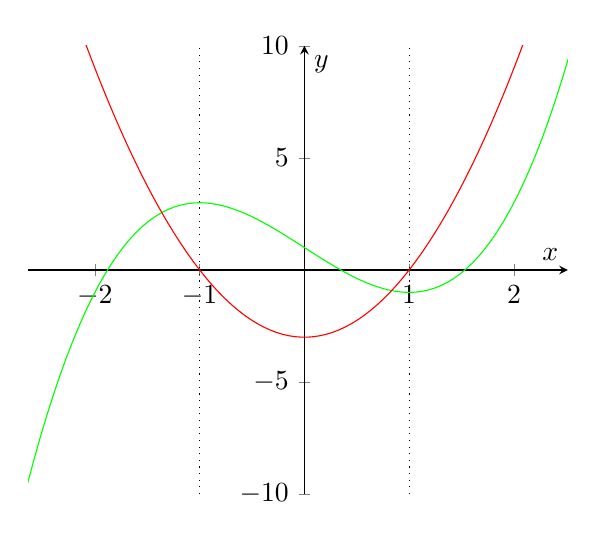
\begin{tikzpicture}
      \begin{axis}[
        axis lines = center,
        xlabel = $ x $,
        ylabel = {$ y $},
        ymax = 10, ymin = -10
      ]
        \addplot[domain = -3:3, color = green, samples = 100] {x^3 - 3*x + 1};
        \addplot[domain = -3:3, color = red, samples = 100] {3*x^2 - 3};
        \draw[style=dotted] (1,-10) -- (1,10);
        \draw[style=dotted] (-1,-10) -- (-1,10);
      \end{axis}
    \end{tikzpicture}}
  \end{center}
\end{ex}

Based on these two examples, we can state the following theorem (but again, we won't prove it here):
\begin{thm}
  If the graph of $ y = f(x) $ has a turning point (maximum or minimum) at $ x = x_0 $, then $ f'(x_0) = 0 $.
\end{thm}

We can look at this from a tangent line perspective as well: at a maximum or a minimum, the graph is `flat' and
so the tangent line is horizontal there --- so the slope of the tangent line and of the function is zero there.

On the other hand, note that $ f'(x_0) =  0 $ does not necessarily imply that $ f $ has a turning point at $ x_0 $.
For example, consider $ y = x^3 $: this function has no turning points, but $ \od{y}{x} = 3x^2 $ is zero at $ (0,0) $.
Places where a function has a zero (or nonexistent) derivative are called critical points.

If the derivative at a critical point exists, but the point is not a maximum or a minimum, then the point is known
as an inflection point. If we look at an entire interval, there may be multiple maxima or minima; the largest maximum
is known as the global maximum of the function on the interval, and the smallest minimum is known as the global minimum
of the function on that interval. Maxima and minima which are not global maxima or minima are known as local maxima
or minima; a function might have no global maxima (take $ y = x^2 $ for example), but on any given closed interval (i.e.
an interval which includes its endpoints) it always attains a local maximum or minimum.

\begin{ex}
  Let us find the critical points of the graph of $ y = 4x^3 - 6x^2 + 2x - 1 $ and classify them. The critical points
  are precisely those places where the slope of the graph is zero --- i.e. the roots of the derivative,
  \begin{displaymath}
    \od{y}{x} = 12x^2 - 12x + 2.
  \end{displaymath}
  Setting the derivative to zero, we can use the quadratic formula to find the two roots are
  \begin{displaymath}
    x = \frac{12 \pm \sqrt{144 - 4 \cdot 12 \cdot 2}}{2 \cdot 12} = \frac{12 \pm \sqrt{48}}{24} = \frac{1}{2} \pm \frac{\sqrt{12}}{6}.
  \end{displaymath}
  Since the cubic has a positive leading coefficient, we know that it will go from $ -\infty $ in the bottom left to $ +\infty $ in the top right,
  and hence the two turning points will be a maximum and a minimum respectively.

  Alternatively, to see this one could note that the derivative is positive to the left of the left-hand turning point, negative between the two,
  and positive again to the right of the right-hand turning point: so the graph changes from increasing, to decreasing, and back to increasing,
  and so we must have a maximum and a minimum in that order.
\end{ex}

Let us look at one final geometric example.
\begin{ex}
  Suppose we have an isosceles triangle $ ABC $, where $ \abs{AB} = \abs{AC} = x $ and $ \abs{BC} = y $. Clearly
  if we spread the edges apart, the area increases and then decreases:
  \begin{center}
    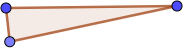
\includegraphics[width=0.18\textwidth]{isos1}
    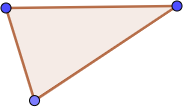
\includegraphics[width=0.18\textwidth]{isos2}
    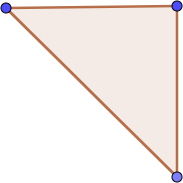
\includegraphics[width=0.18\textwidth]{isos3}
    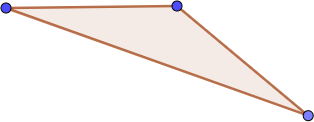
\includegraphics[width=0.18\textwidth]{isos4}
    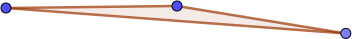
\includegraphics[width=0.18\textwidth]{isos5}
  \end{center}

  The area of the isosceles triangle is given by
  \begin{displaymath}
    A = \frac{1}{2} \times y \times \sqrt{x^2 - \frac{y^2}{4}}.
  \end{displaymath}
  Now, we can't actually take the derivative of this function this year --- but area is always positive, so the minimum of the area squared
  will be at the same place as the minimum of the area. Hence we want to minimise
  \begin{displaymath}
    A^2 = \frac{1}{4}y^2\left(x^2 - \frac{y^2}{4}\right) = \frac{1}{4} x^2 y^2 - \frac{1}{16}y^4
  \end{displaymath}
  with respect to $ y $ (since $ x $ is fixed).

  We have that $ \od{A^2}{y} = (1/2) x^2 y - (1/4)y^3 $; setting this to zero, we have that $ x^2 y = (1/2)y^3 $. Since we know
  that $ y \neq 0 $ (that corresponds to a minimum, not a maximum) we can divide through, and so $ x^2 = (1/2) y^2 $ --- so the
  minimum occurs when $ y = x\sqrt{2} $.

  Of course, this corresponds to the situation where the angle between the two equal sides is a right angle (for then $ \sqrt{x^2 + x^2} = x\sqrt{2} $, as
  we just found is the case) --- this is what we would expect from the symmetry of the triangle and from playing around with different pictures of
  an isoceles triangle. If we draw the triangle inside a circle, it is the halfway point between the two zero-area possibilities.
\end{ex}

\clearpage
\subsection*{Questions}
\begin{questions}
  \question Consider the function graphed below.
            \begin{center}
              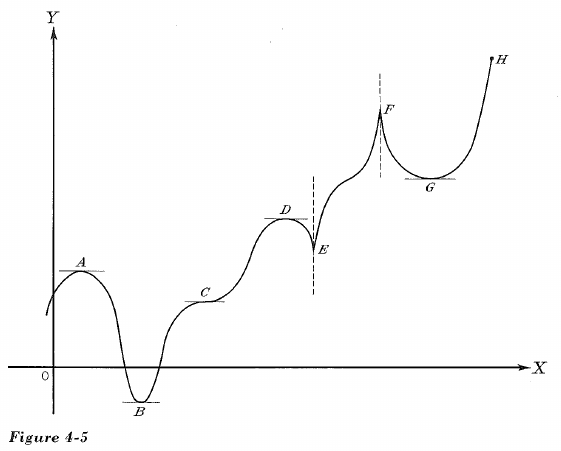
\includegraphics[width=0.6\textwidth]{extrema}
            \end{center}
            For each point $ A $ to $ H $:
            \begin{itemize}
              \item Explain why the point is a critical point of the function by either giving the slope of the function at that point, or explaining
                    why the derivative does not exist at that point.
              \item Label the point as an inflection point, a maximum, or a minimum.
              \item If the point is a maximum or a minimum, label it as either local or global.
            \end{itemize}
  \question Sketch graphs with the following properties:
    \begin{parts}
      \part A maximum at $ x = 3 $ and a minimum at $ x = 6 $.
      \part No maximums or minimums, but critical points at $ x = 2 $ and $ x = 4 $.
      \part Maximums at $ x = 2 $ and $ x = 4 $ but no minimums.
    \end{parts}
  \question Find the maximum and minimum points of the function $ g $ defined by $ g(x) = 2x^3 + x^2 + 2x $.
  \question The function $ F $, where $ F(x) = x^{\frac{4}{5}} (x - 4)^2 $, has critical points at $ x = 0 $, $x = \frac{8}{7}$, and $ x = 4 $. Classify
            each one as a maximum, a minimum, or neither.
  \question Show that the turning points of $ y = x^4 - x^2 $ are, alternately, minimum, maximum, and minimum.
  \question Find the extreme values (if any) of the following functions of $ x $:
    \begin{multicols}{2}
    \begin{parts}
      \part $ y = x^5 $
      \part $ y = \frac{1}{x} $
      \part $ y = x^2 - 1 $
      \part $ y = 2x^3 - 21x^2 + 72x + 18 $
      \part $ f(x) = x^{10} - 4 $
      \part $ y = \frac{1}{\sqrt{x}} + x^2 $
      \part $ y = x^3 - x - 1 $
      \part $ y = x^3 - x^2 + x - 1 $
      \part $ f(x) = \frac{1}{x} + x - x^2 $
      \part $ y = 16 $
      \part $ y = \frac{x^{-2} + x^2}{2x} $
      \part $ x = \frac{y - 2}{x + 3} $
    \end{parts}
    \end{multicols}
  \question Find the maximum value of the derivative of $ 2x^2 - x^3 $.
  \question Prove that the function $ \varphi $ given by $ \varphi(x) = \frac{x^{101}}{101} + \frac{x^{51}}{51} + x + 1 $ has no extreme values.
  \question Show that:
    \begin{parts}
      \part $ y = x^4 + 3x^3 - x^2 - x + 20 $ does not pass through the $ x$-axis.
      \part $ x^3 - 5x + 100 = 0 $ has only one real solution.
      \part $ x^3 - x^2 - x + 1 $ has exactly two roots.
    \end{parts}
  \question A farmer needs to create a rectangular field with a fence. He has \SI{500}{\metre} of fencing available, and a building
            is on one side of the field (so that side does not need fencing). Determine the dimensions of the field to enclose the
            greatest area.
  \question Suppose that a rectangle has perimeter $ p $. Show that if the rectangle is to have the greatest possible area then it
            must be a square.
  \question Find the maximum value of $ y = -x^2 + 6x - 5 $, both
    \begin{parts}
      \part \emph{without} calculus; and
      \part \emph{with} calculus.
    \end{parts}
  \question Find $ k $ so that $ y = x^3 + kx^2 + x + 1 $ has (a) two, (b) one, and (c) zero turning points.
  \question The graph of $ f(x) = x^3 + ax^2 + bx + 2 $ has turning points when $ x = -1 $ and $ x = 3 $. Find the values of $ a $ and $ b $.
  \question Prove that the graph of $ y = x^3(3 - x) $ has a local maximum when $ x = \frac{9}{4} $. Carefully justify that the turning point
            \emph{is} a local maximum.
  \question Find the maximum volume of an open box (i.e. a box with base and sides, but no lid) that can be made from a rectangular piece of
            cardboard measuring \SI{20}{\centi\metre} by \SI{30}{\centi\metre} by removing the corner squares and folding along the dotted
            lines. Carefully justify that this is the maximum volume.
            \begin{center}
              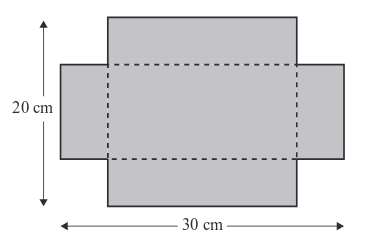
\includegraphics[width=0.3\textwidth]{box}
            \end{center}
  \question In an area surrounding a farming airstrip there is a height restriction for
            fireworks of \SI{50}{\metre}. The height $ h $ metres above the ground reached
            by a firework $ t $ seconds after it is fired can be modelled by the function
            \begin{equation}
              h = 20t - 5t^2.
            \end{equation}
            Will the firework break the \SI{50}{\metre} limit?
  \question By noting that the derivative changes from positive to negative at a maximum, and from negative to positive at a minimum, suggest
            a criteria for classifying turning points using the second derivative.
\end{questions}

\end{document}
